\chapter{Results}
\section{Bengio Style Curricula}
As covered in our methodology section we implemented the Bengio Style(referred to as BS) curricula across the two sizes of wikitext corpuses. We evaluate model performance on the validation portion at the end of each epoch and once the model has trained for 10 epochs we evaluate on the JIANT implemented GLUE baseline. Unless other called the glue measure is accuracy
\begin{table}[!h]
\begin{tabular}{|l|l|l|l|l|}
\hline 
Epochs & baseline wiki-2 & bs wiki-2 & bs wiki-103 & baseline wiki-103 \\ \hline \hline  
1  & 620.45544 & 758.29285 & 227.65094 & 83.05149  \\ \hline 
2  & 451.85522 & 507.58508 & 138.29044 & 56.865345 \\ \hline 
3  & 358.74582 & 445.0215  & 113.23114 & 48.632687 \\ \hline  
4  & 303.83347 & 424.0015  & 100.1231  & 44.216614 \\ \hline  
5  & 241.15233 & 364.40637 & 92.03778  & 41.57386  \\ \hline  
6  & 221.38237 & 395.8324  & 90.143585 & 39.798542 \\ \hline 
7  & 195.55809 & 213.29416 & 39.72011  & 38.54776  \\ \hline  
8  & 168.30266 & 181.99895 & 38.672005 & 37.64779  \\ \hline 
9  & 162.16602 & 163.70233 & 37.66034  & 37.009693 \\ \hline 
10 & 151.25607 & 153.26689 & 37.029747 & 36.412056 \\ \hline 
\end{tabular}
\label{table:corpuscurriculaperplexity}
\caption{Model Perplexity on validation portion of the train corpus. BS approaches the baseline method without ever passing it.}
\end{table}
As seen in figure 4.1 we see that the baseline method implementations outperform the BS across the entire training regime. Initially, while the model is training on the limited corpus it performs worse on the validation set. As the model reaches the original training data the resulting embeddings reach close to the baseline perplexity but are never able to pass the baseline method. By the 7th epoch both methods have virtually identical perplexities. Another interesting trend is the fact that on the small corpus when the full corpus is introduced(epoch 6) the validation perplexity briefly increases. Final observation is that the baseline method reaches low perplexity on large corpus much faster than the bs method. The baseline method is able to achieve a perplexity under 100 by the end of the first epoch while the BS method cannot do so until the end of the 5th. \\
\begin{figure}[h]
\centering
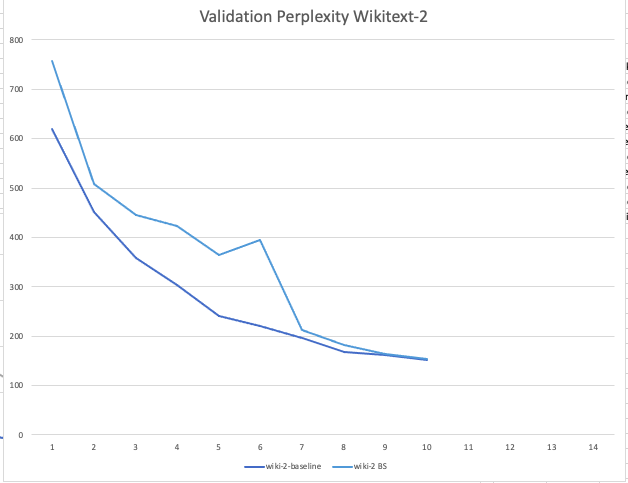
\includegraphics[width=10cm, height=10cm]{Thesis/images/bs-wiki2-valid.png}
\caption{GLUE results for BS vs baseline.}
\end{figure}
\begin{figure}[h]
\centering
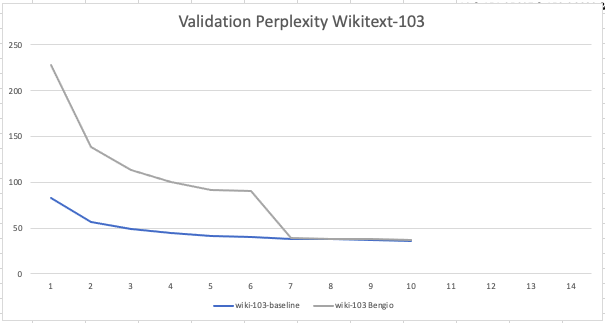
\includegraphics[width=10cm, height=10cm]{Thesis/images/bs-wiki103-valid.png}
\caption{GLUE results for BS vs baseline.}
\end{figure}
\begin{sidewaystable}[htbp]
  \resizebox{0.7\textwidth}{!}{\begin{minipage}{\textwidth}
\begin{tabular}{|l|l|l|l|l|l|l|l|l|l|l|l|l|l|l|l|}
\hline
Corpus & Method & Score & Cola(MCC) & SST & MRPC(F1) & MRPC & STS-B(Pear) & STS-B(Spear) & QQP(F1) & QQP & MNLI & QNLI & RTE & WNLI & Diagnostic \\ \hline
wikitext-103 & NC & 0.671 & 0.281 & 0.862 & 0.866 & 0.801 & 0.765 & 0.773 & 0.716 & 0.763 & 0.644 & 0.761 & 0.61 & 0.535 & 0.139 \\\hline
wikitext-103 & BS & 0.657 & 0.254 & 0.852 & 0.875 & 0.816 & 0.794 & 0.793 & 0.738 & 0.785 & 0.662 & 0.719 & 0.588 & 0.437 & 0.162 \\\hline
wikitext-2 & BS & 0.607 & 0.06 & 0.742 & 0.854 & 0.789 & 0.683 & 0.684 & 0.697 & 0.745 & 0.566 & 0.726 & 0.581 & 0.563 & 0.119 \\\hline
wikitext-2 & NC & 0.59 & 0 & 0.7 & 0.846 & 0.775 & 0.661 & 0.663 & 0.701 & 0.753 & 0.585 & 0.717 & 0.542 & 0.563 & 0.13 \\\hline
billion word & NC & 0.595 & 0 & 0.852 & 0.823 & 0.711 & 0.547 & 0.562 & 0.733 & 0.765 & 0.671 & 0.719 & 0.48 & 0.563 & 0.155 \\ \hline
\end{tabular}
\end{minipage}}
\caption{GLUE results for BS vs baseline.\\ Model performance is better with BS when corpus is small but as corpus scales baseline method out performs BS}
\label{tab:glue-corpus}}
\end{sidewaystable}
When we evaluate the effect of the curricula looking at glue \ref{tab:glue-corpus} we see a few interesting results. First off we that the pubic elmo implementation does surprisingly worse on the GLUE dataset. It is unclear why this is and we will not focus on this further. Next we find that when the training corpus is small the BS implementation our performs the baseline method. As the corpus size grows the baseline performance passes all other methods. There is high variability in each tasks such that STS-B and the Diagnostic tests are much better with the BS system while MCC, WNLI, and RTE are much better in baseline method. If we exclude WNLI the BS methods outperform the baseline methods by a wide margin. We also are able to observe that there are various tasks that the small corpus models cannot learn as both wikitext-2 models achieve 0 on COLA.
\section{Competence Based Curricula}
Now we move onto the results of the competence curricula. In this section DEP represents dependency parse depth, POS represents part of speech diversity, CC represents competence curricula.
\subsection{Wikitext-2}
Looking at performance on the small corpus \ref{tab:wikitext2-line-perplexity} and \ref{tab:wikitext2-sentence-perplexity} we see that all the curricula methods start to over fit on the train corpus after about 16 of the 24 epochs(which equates to when the curricula finishes). Despite seeing over fitting we see that POS and DEP generally learn some of the lowest perplexity on the validation set. Looking at the difference between sentence and line level training we see a closer grouping in model performance distribution which we attribute to common sentence level structure. Finally, we see that the best performance is actually achieved by the non curricula baseline(competence set to 1) with a perplexity of 770 followed by Random 2105 both of which are way higher than the baseline score of 151.\\
As we move our focus to GLUE we see a very different picture as the curriculum methods generally outperform the baselines by a wide margin. We see that models do not seem to learn any type of representation that can be used by WNLI as those results are all virtually identical. Surprisingly it does not seem that a method that performs well in sentence based training achieves a similar result in line based training and we do not believe a strong generalization can be made about the effects of the two corpus methods. The final point to observe that that nearly every curricula method outperforms the baseline implementation with even the random curricula performing 2nd best. We believe the results of the corpus based curricula and the competence curricula support the hypothesis that curricula methods are useful when the training corpus is small. 
\begin{table}[]
\centering
\resizebox{\textwidth}{!}{
\begin{tabular}{|l|l|l|l|l|l|l|l|l|}
\hline
Batches & Baseline & Random & Dependency & Part of Speech & Unigram & Bigram & Trigram & Length \\ \hline
0 & 19498.28 & 21163.44 & 26654.95 & 26528.35 & 22053.12 & 19535.65 & 20830.92 & 29933.74 \\ \hline
100 & 5600.459 & 5461.039 & 5730.613 & 5215.405 & 5412.148 & 5164.017 & 5130.01 & 6159.207 \\ \hline
200 & 8412.964 & 5335.186 & 4173.729 & 4526.756 & 4801.211 & 4104.102 & 4100.64 & 5091.564 \\ \hline
300 & 10206.76 & 5121.969 & 4350.757 & 4552.211 & 5111.258 & 4242.258 & 5154.742 & 4209.991 \\ \hline
400 & 9694.969 & 4656.295 & 4411.583 & 4181.944 & 4576.212 & 4606.979 & 4085.841 & 4266.357 \\ \hline
500 & 4263.702 & 4187.064 & 3975.314 & 4448.919 & 4315.669 & 3466.285 & 3425.474 & 6061.277 \\ \hline
600 & 4637.823 & 4007.23 & 3804.034 & 5325.821 & 3865.498 & 3853.12 & 3574.217 & 5577.375 \\ \hline
700 & 3670.097 & 4142.923 & 3831.932 & 3942.862 & 9677.842 & 3230.582 & 3502.653 & 4219.224 \\ \hline
800 & 3221.346 & 3970.763 & 3749.825 & 4645.618 & 4742.95 & 2954.3 & 3138.186 & 4247.958 \\ \hline
900 & 3959.106 & 5503.046 & 4688.382 & 5068.281 & 3871.681 & 3856.12 & 12232.67 & 4298.991 \\ \hline
1000 & 3132.26 & 8124.751 & 4383.869 & 4416.356 & 4699.026 & 3397.773 & 8652.374 & 3856.153 \\ \hline
1100 & 13849.47 & 7308.988 & 4047.798 & 4257.96 & 6621.724 & 5047.275 & 5068.213 & 5205.368 \\ \hline
1200 & 6503.515 & 5181.124 & 4269.158 & 7781.854 & 17770.95 & 3666.078 & 10005.95 & 4551.86 \\ \hline
1300 & 7178.955 & 19722.45 & 5696.292 & 3884.615 & 14288.98 & 8585.893 & 10586.63 & 4248.825 \\ \hline
1400 & 5806.94 & 7711.413 & 3276.619 & 4795.949 & 11649.69 & 14055.36 & 9180.324 & 4275.567 \\ \hline
1500 & 7896.527 & 9227.372 & 6222.824 & 4230.453 & 7551.371 & 12330.95 & 57175.42 & 5575.008 \\ \hline
1600 & 21873.66 & 36947.88 & 4324.498 & 7872.976 & 14629.82 & 12650.03 & 23212.86 & 5090.137 \\ \hline
1700 & 12979.71 & 20851.81 & 5498.242 & 5195.954 & 5852.289 & 28631.84 & 56772.43 & 5290.866 \\ \hline
1800 & 34403.65 & 24371.06 & 4613.688 & 6938.421 & 17223.34 & 10833.46 & 56383.88 & 5559.394 \\ \hline
1900 & 45148.42 & 12774.94 & 4005.43 & 7535.285 & 21746.75 & 32077.18 & 50338.7 & 3713.533 \\ \hline
2000 & 28062.45 & 62992.67 & 4582.964 & 6047.258 & 26790.6 & 29896.4 & 25035.54 & 6571.44 \\ \hline
2100 & 28706.4 & 105545.6 & 3806.545 & 8146.35 & 42521.56 & 68461.61 & 36110.3 & 5294.52 \\ \hline
2200 & 42284.38 & 62399.3 & 5332.897 & 4722.252 & 19101.4 & 78817.77 & 111061.6 & 8789.567 \\ \hline
2300 & 211236.3 & 89274.6 & 4591.32 & 6133.123 & 60930.05 & 57298.29 & 53007.47 & 7117.323 \\ \hline
2400 & 23207.46 & 115620.8 & 4978.687 & 5435.751 & 44079.81 & 49065.99 & 81409.19 & 6686.693 \\ \hline
\end{tabular}
}
\caption{Perplexity of each curricula trained on line based wikitext on validation corpus measured every 100 batches}
\label{tab:wikitext2-line-perplexity}
\end{table}

\begin{figure}[h]
\centering
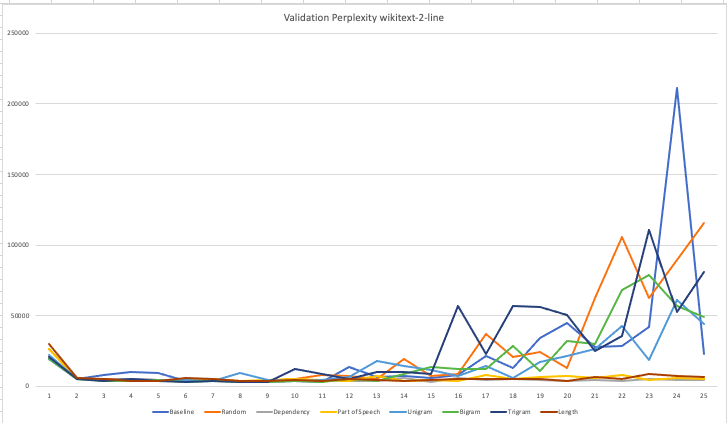
\includegraphics[width=10cm, height=10cm]{Thesis/images/wiki2-line-valid.png}
\caption{Perplexity on wiki2-line corpus. DEP, POS, and LEN avoid the overfitting the other models see}
\end{figure}

\begin{table}[]
\centering
\resizebox{\textwidth}{!}{%
\begin{tabular}{|l|l|l|l|l|l|l|l|l|}
\hline
Batches & Baseline & Random & Dependency & Part of Speech & Unigram & Bigram & Trigram & Length \\ \hline
0 & 19577 & 18972.3 & 21636.473 & 25085.371 & 17233.63 & 16562.04 & 16953.24 & 25580.67 \\ \hline
100 & 4393.4 & 3869.01 & 4907.4766 & 5089.3213 & 4227.456 & 3895.485 & 5203.784 & 5679.227 \\ \hline
200 & 3775.8 & 3342.43 & 3766.6887 & 3795.3662 & 3193.679 & 3014.929 & 3285.696 & 5670.292 \\ \hline
300 & 3193.5 & 2855.56 & 3518.257 & 3350.3381 & 3022.722 & 2862.637 & 10340.28 & 7913.436 \\ \hline
400 & 3018 & 2868.06 & 3079.2112 & 3235.9043 & 2984.732 & 2797.256 & 2898.078 & 4154.833 \\ \hline
500 & 2629.8 & 2624.77 & 3339.034 & 3249.0745 & 2615.482 & 2638.166 & 2932.65 & 2693.087 \\ \hline
600 & 2751.3 & 2482.34 & 2926.965 & 2851.3337 & 2597.397 & 2542.316 & 2572.945 & 2762.114 \\ \hline
700 & 2538.6 & 2377.76 & 2814.3276 & 3095.3398 & 2438.547 & 2426.895 & 2399.556 & 2432.863 \\ \hline
800 & 3605.3 & 2241.75 & 2780.0137 & 3009.666 & 3130.137 & 2377.921 & 2476.211 & 2709.775 \\ \hline
900 & 2679 & 2297.78 & 2464.8281 & 2462.9426 & 4788.499 & 2485.33 & 2421.764 & 2963.076 \\ \hline
1000 & 3212.4 & 2219.75 & 2665.2764 & 2486.0417 & 2088.218 & 2745.638 & 2329.685 & 2468.642 \\ \hline
1100 & 3965.8 & 2257.58 & 10348.93 & 2716.1235 & 2225.749 & 2263.412 & 2619.83 & 2386.155 \\ \hline
1200 & 2557 & 2224.1 & 3332.5085 & 2176.2024 & 2086.037 & 2821.298 & 2512.837 & 2055.139 \\ \hline
1300 & 2566.7 & 2505.48 & 2912.2942 & 2439.959 & 2668.968 & 2386.25 & 2376.939 & 2844.38 \\ \hline
1400 & 4251.9 & 2659.05 & 3528.9463 & 2964.2732 & 2541.053 & 2565.921 & 2829.178 & 2446.484 \\ \hline
1500 & 2974.5 & 2815.76 & 2924.3967 & 2067.4797 & 3674.223 & 2774.171 & 2343.067 & 2960.37 \\ \hline
1600 & 2915.3 & 2344.01 & 2849.28 & 2534.103 & 3890.443 & 3291.204 & 2685.646 & 3916.598 \\ \hline
1700 & 2847.2 & 2127.63 & 5314.9077 & 2186.36 & 3038.41 & 3183.71 & 2816.234 & 2621.306 \\ \hline
1800 & 2747.2 & 2285.29 & 2729.2192 & 2487.4993 & 2781.731 & 2755.068 & 2685.075 & 2596.71 \\ \hline
1900 & 3222.8 & 2440.04 & 2387.6428 & 2464.5767 & 3036.206 & 2939.755 & 2961.87 & 3006.224 \\ \hline
2000 & 3432.1 & 2423.35 & 2498.7942 & 2584.4092 & 2965.91 & 2836.161 & 2218.454 & 2221.723 \\ \hline
2100 & 3438.4 & 2001.77 & 2103.243 & 3023.273 & 3039.94 & 2557.588 & 2440.281 & 2958.65 \\ \hline
2200 & 2597.5 & 2516.39 & 2807.2107 & 3113.2212 & 2539.777 & 2650.921 & 2384.331 & 2922.845 \\ \hline
2300 & 2537.7 & 2572.49 & 2737.5596 & 2898.6365 & 3100.773 & 2493.721 & 2449.759 & 2993.907 \\ \hline
2400 & 3433.7 & 2633.99 & 2596.0078 & 2330.572 & 2583.728 & 2229.844 & 2207.221 & 2361.876 \\ \hline
2500 & 3063.9 & 2835.72 & 1969.3733 & 2286.7202 & 2515.244 & 2056.117 & 2092.182 & 3337.922 \\ \hline
2600 & 3235.2 & 2638.41 & 4091.7915 & 2449.3496 & 3334.162 & 2431.215 & 2069.936 & 3580.122 \\ \hline
2700 & 4040.3 & 2670.14 & 3125.7693 & 2753.1929 & 3107.351 & 2691.088 & 2656.51 & 4305.21 \\ \hline
2800 & 3402.3 & 2347.04 & 5570.7563 & 2362.6565 & 2062.797 & 2586.205 & 2425.246 & 3611.754 \\ \hline
2900 & 5388.1 & 2740.16 & 4000.6243 & 3194.3093 & 2790.644 & 2407.481 & 2207.875 & 4251.675 \\ \hline
3000 & 5389.1 & 2568.82 & 11589.234 & 3652.8022 & 2783.052 & 2784.212 & 2332.16 & 3563.234 \\ \hline
3100 & 4227.3 & 3012.2 & 3253.4585 & 3206.2273 & 2920.262 & 3337.26 & 2850.718 & 2102.434 \\ \hline
3200 & 3962.9 & 3157.9 & 10045.327 & 4041.8535 & 3573.764 & 2864.314 & 2191.798 & 3055.313 \\ \hline
3300 & 5547.2 & 2583.23 & 17333.396 & 3213.1606 & 2899.022 & 2394.718 & 2577.445 & 2699.329 \\ \hline
3400 & 7155.4 & 3601.26 & 3040.4277 & 3099.2976 & 3455.618 & 2837.321 & 2653.487 & 3373.731 \\ \hline
3500 & 5882.7 & 3813.07 & 16560.428 & 2756.5728 & 4385.529 & 2440.946 & 3067.075 & 2999.78 \\ \hline
3600 & 4887.4 & 2530.43 & 9361.988 & 2919.6719 & 3249.393 & 2523.844 & 2807.685 & 2630.625 \\ \hline
3700 & 6196.1 & 2383.66 & 20497.451 & 2655.2168 & 4421.092 & 2611.211 & 3142.592 & 2940.323 \\ \hline
3800 & 5810.9 & 3164.84 & 17406.648 & 3329.6848 & 5049.87 & 3314.212 & 3773.563 & 3204.518 \\ \hline
3900 & 5575.6 & 2112.18 & 11576.83 & 2928.0552 & 3045.523 & 2490.426 & 2244.873 & 2624.535 \\ \hline
\end{tabular}
}
\caption{Perplexity of each curricula trained on line based wikitext-2 on validation corpus measured every 100 batches}
\label{tab:wikitext2-sentence-perplexity}
\end{table}


\begin{figure}[h]
\centering
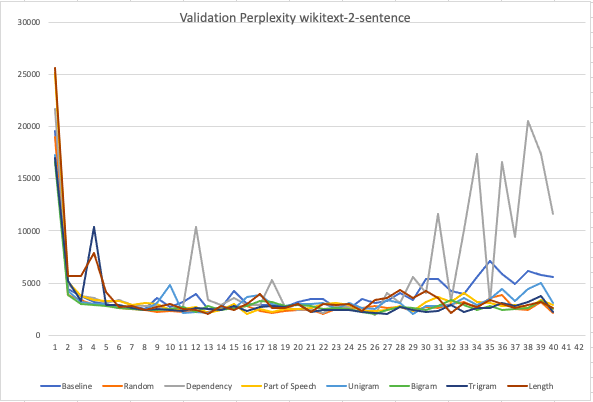
\includegraphics[width=10cm, height=10cm]{Thesis/images/wiki2-sentence-valid.png}
\caption{Model perplexity on wikitext2-setnence by curricula. Note DEP and trigram overfitting.}
\end{figure}

\begin{sidewaystable}[htbp]
  \resizebox{0.7\textwidth}{!}{\begin{minipage}{\textwidth}
\begin{tabular}{|l|l|l|l|l|l|l|l|l|l|l|l|l|l|l|l|l|}
\hline
Corpus & Method & Curricula & Score & Cola(MCC) & SST & MRPC(F1) & MRPC & STS-B(Pear) & STS-B(Spear) & QQP(F1) & QQP & MNLI & QNLI & RTE & WNLI & Diagnostic \\ \hline
sentence & cc & bigram & 0.644556 & 0.188 & 0.79 & 0.844 & 0.775 & 0.732 & 0.733 & 0.742 & 0.788 & 0.617 & 0.766 & 0.57 & 0.563 & 0.131 \\ \hline
sentence & cc & random & 0.643667 & 0.21 & 0.78 & 0.847 & 0.779 & 0.715 & 0.712 & 0.744 & 0.791 & 0.616 & 0.76 & 0.57 & 0.563 & 0.143 \\ \hline
sentence & cc & unigram & 0.639833 & 0.209 & 0.755 & 0.861 & 0.799 & 0.731 & 0.731 & 0.733 & 0.778 & 0.613 & 0.757 & 0.545 & 0.563 & 0.135 \\ \hline
sentence & cc & POS & 0.637111 & 0.207 & 0.765 & 0.849 & 0.777 & 0.714 & 0.714 & 0.727 & 0.781 & 0.606 & 0.745 & 0.567 & 0.563 & 0.134 \\ \hline
sentence & cc & DEP & 0.636 & 0.175 & 0.792 & 0.863 & 0.797 & 0.721 & 0.72 & 0.727 & 0.786 & 0.613 & 0.749 & 0.567 & 0.521 & 0.137 \\ \hline
line & cc & DEP & 0.631944 & 0.19 & 0.727 & 0.85 & 0.782 & 0.708 & 0.704 & 0.735 & 0.782 & 0.598 & 0.748 & 0.581 & 0.563 & 0.118 \\ \hline
line & cc & unigram & 0.628278 & 0.175 & 0.768 & 0.856 & 0.782 & 0.675 & 0.674 & 0.738 & 0.792 & 0.598 & 0.746 & 0.56 & 0.549 & 0.132 \\ \hline
line & cc & trigram & 0.627444 & 0.152 & 0.761 & 0.838 & 0.762 & 0.695 & 0.691 & 0.73 & 0.782 & 0.616 & 0.764 & 0.542 & 0.563 & 0.144 \\ \hline
sentence & cc & trigram & 0.626278 & 0.172 & 0.788 & 0.833 & 0.779 & 0.73 & 0.731 & 0.744 & 0.796 & 0.62 & 0.761 & 0.552 & 0.437 & 0.137 \\ \hline
line & cc & length & 0.625444 & 0.185 & 0.748 & 0.844 & 0.77 & 0.658 & 0.654 & 0.725 & 0.783 & 0.601 & 0.748 & 0.567 & 0.563 & 0.128 \\ \hline
line & cc & baseline & 0.621389 & 0.148 & 0.747 & 0.836 & 0.77 & 0.706 & 0.705 & 0.734 & 0.78 & 0.612 & 0.719 & 0.538 & 0.563 & 0.121 \\ \hline
line & cc & bigram & 0.615833 & 0.175 & 0.768 & 0.856 & 0.782 & 0.675 & 0.674 & 0.738 & 0.792 & 0.598 & 0.746 & 0.56 & 0.437 & 0.132 \\ \hline
line & cc & random & 0.614056 & 0 & 0.763 & 0.847 & 0.775 & 0.699 & 0.699 & 0.721 & 0.784 & 0.611 & 0.749 & 0.578 & 0.563 & 0.143 \\ \hline
line & bs & N/A & 0.607111 & 0.06 & 0.742 & 0.854 & 0.789 & 0.683 & 0.684 & 0.697 & 0.745 & 0.566 & 0.726 & 0.581 & 0.563 & 0.119 \\ \hline
line & cc & POS & 0.606778 & 0 & 0.737 & 0.842 & 0.77 & 0.663 & 0.66 & 0.712 & 0.771 & 0.61 & 0.75 & 0.592 & 0.563 & 0.155 \\ \hline
sentence & cc & baseline & 0.591056 & 0.069 & 0.768 & 0.847 & 0.765 & 0.728 & 0.731 & 0.722 & 0.758 & 0.5 & 0.718 & 0.538 & 0.451 & 0.107 \\ \hline
line & baseline & N/A & 0.589611 & 0 & 0.7 & 0.846 & 0.775 & 0.661 & 0.663 & 0.701 & 0.753 & 0.585 & 0.717 & 0.542 & 0.563 & 0.13 \\ \hline
sentence & cc & length & 0.527889 & -0.006 & 0.75 & 0.805 & 0.674 & 0.708 & 0.71 & 0.537 & 0.682 & 0.326 & 0.51 & 0.592 & 0.521 & 0.008 \hline
\end{tabular}
\end{minipage}}
\caption{GLUE results for BS vs baseline.\\ Model performance is better with BS when corpus is small but as corpus scales baseline method out performs BS}
}
\label{tab:wiki2-glue}

\end{sidewaystable}

\subsection{wikitext-103}
As we scale to the larger corpus we find that some trends hold while others do not. Looking at the results in \ref{wikitext-103-line} and \ref{tab:wikitext-103-sentence} we can see that similar to the smaller corpus none of the curricula learned methods are able to learn a representation that transfers well to the validation set. Unlike the non curricula methods which achieve a perplexity of 36 none of the curricula methods ever learn a representation with a perplexity under one thousand. We note that similar to the smaller corpus the ngram methods behave in a similar pattern and performance is quite comparable. Similar to the performance on the small corpus DEP, LEN, and POS demonstrate a slow and steady improvement in perplexity as their training continues. We also see the behavior in highly volatile perplexity changes scale from the small dataset to the large dataset which is surprising. When joined with the behavior
Looking at the result on the transfer tasks as measured by GLUE \ref{glue-wiki-103} we find that the trends we say in the smaller corpus no longer hold. The best model in terms of transfer learning is the non curriculum model. This baseline method not only out performs on the overall score but also out performs every other model on tasks like CoLA where the score is nearly 20\% better. Surprisingly after the baseline method it appears the trigram curricula appear to generate the best transfer task as both sentence and line based methods 2nd and 3rd best models. We also note that some of the best performing curricula are also those models that had some of the highest perplexities on the training task.

\begin{table}[]
\centering
\resizebox{\textwidth}{!}{%
\begin{tabular}{|l|l|l|l|l|l|l|l|l|l|l|l|l|l|l|l|l|}
\hline
Corpus style & Train Method & Competence Method & Score & Cola(MCC) & SST & MRPC(F1) & MRPC & STS-B(Pear) & STS-B(Spear) & QQP(F1) & QQP & MNLI & QNLI & RTE & WNLI & Diagnostic \\ \hline
line & baseline & N/A & 0.670556 & 0.281 & 0.862 & 0.866 & 0.801 & 0.765 & 0.773 & 0.716 & 0.763 & 0.644 & 0.761 & 0.61 & 0.535 & 0.139 \\ \hline
sentence & Competence Curriculum & trigram & 0.665722 & 0.208 & 0.857 & 0.865 & 0.806 & 0.79 & 0.79 & 0.733 & 0.779 & 0.658 & 0.757 & 0.567 & 0.563 & 0.136 \\ \hline
line & Competence Curriculum & trigram & 0.664722 & 0.207 & 0.854 & 0.871 & 0.804 & 0.781 & 0.782 & 0.752 & 0.799 & 0.655 & 0.767 & 0.556 & 0.549 & 0.144 \\ \hline
sentence & Competence Curriculum & unigram & 0.663778 & 0.19 & 0.856 & 0.861 & 0.797 & 0.784 & 0.784 & 0.747 & 0.791 & 0.654 & 0.773 & 0.556 & 0.563 & 0.14 \\ \hline
sentence & Competence Curriculum & baseline & 0.663278 & 0.19 & 0.845 & 0.878 & 0.824 & 0.767 & 0.768 & 0.748 & 0.788 & 0.651 & 0.746 & 0.588 & 0.563 & 0.14 \\ \hline
line & Competence Curriculum & baseline & 0.663056 & 0.214 & 0.826 & 0.865 & 0.804 & 0.766 & 0.766 & 0.747 & 0.789 & 0.643 & 0.772 & 0.581 & 0.563 & 0.145 \\ \hline
sentence & Competence Curriculum & random & 0.661444 & 0.203 & 0.843 & 0.87 & 0.806 & 0.778 & 0.779 & 0.74 & 0.789 & 0.644 & 0.745 & 0.574 & 0.563 & 0.151 \\ \hline
sentence & Competence Curriculum & length & 0.658556 & 0.229 & 0.827 & 0.867 & 0.804 & 0.765 & 0.766 & 0.747 & 0.783 & 0.642 & 0.762 & 0.538 & 0.563 & 0.135 \\ \hline
line & Bengio curricula & N/A & 0.656944 & 0.254 & 0.852 & 0.875 & 0.816 & 0.794 & 0.793 & 0.738 & 0.785 & 0.662 & 0.719 & 0.588 & 0.437 & 0.162 \\
line & Competence Curriculum & bigram & 0.656278 & 0.18 & 0.826 & 0.854 & 0.792 & 0.77 & 0.77 & 0.753 & 0.794 & 0.645 & 0.766 & 0.56 & 0.563 & 0.137 \\
line & Competence Curriculum & length & 0.656 & 0.212 & 0.82 & 0.851 & 0.782 & 0.768 & 0.767 & 0.734 & 0.788 & 0.634 & 0.752 & 0.578 & 0.563 & 0.135 \\ \hline
line & Competence Curriculum & unigram & 0.653611 & 0.194 & 0.823 & 0.857 & 0.789 & 0.755 & 0.754 & 0.752 & 0.794 & 0.625 & 0.753 & 0.574 & 0.563 & 0.125 \\ \hline
line & Competence Curriculum & random & 0.652333 & 0.179 & 0.836 & 0.861 & 0.789 & 0.772 & 0.774 & 0.753 & 0.797 & 0.64 & 0.772 & 0.578 & 0.493 & 0.139 \\ \hline
line & Competence Curriculum & part of speech diversity & 0.649056 & 0.163 & 0.827 & 0.861 & 0.794 & 0.756 & 0.757 & 0.754 & 0.791 & 0.63 & 0.732 & 0.57 & 0.563 & 0.138 \\ \hline
sentence & Competence Curriculum & bigram & 0.648611 & 0.195 & 0.859 & 0.867 & 0.799 & 0.784 & 0.785 & 0.736 & 0.772 & 0.651 & 0.754 & 0.599 & 0.408 & 0.132 \\ \hline
line & Competence Curriculum & dependency parse depth & 0.644389 & 0.231 & 0.846 & 0.856 & 0.779 & 0.776 & 0.776 & 0.746 & 0.786 & 0.637 & 0.761 & 0.542 & 0.423 & 0.137 \\ \hline
sentence & Competence Curriculum & part of speech diversity & 0.639889 & 0.114 & 0.794 & 0.853 & 0.772 & 0.775 & 0.774 & 0.74 & 0.782 & 0.624 & 0.738 & 0.578 & 0.563 & 0.108 \\ \hline
sentence & Competence Curriculum & dependency parse depth & 0.5865 & -0.04 & 0.842 & 0.805 & 0.679 & 0.786 & 0.789 & 0.682 & 0.73 & 0.321 & 0.757 & 0.614 & 0.549 & 0.038 \\ \hline
\end{tabular}
}
\caption{GLUE performance on models trained with wikitext-103}
\label{tab:glue-wiki-103}
\end{table}

\begin{table}[]
\centering
\resizebox{\textwidth}{!}{
\begin{tabular}{|l|l|l|l|l|l|l|l|l|}
\hline
Batches & Baseline & Random & Dependency & Part of Speech & Unigram & Bigram & Trigram & Length \\ \hline
0 & 172216.9 & 165166.4 & 207358.9 & 215021.8 & 161038.8 & 172513.9 & 154467.2 & 225595.5 \\ \hline
100 & 17752.13 & 14454.38 & 18175.47 & 22662.42 & 16281.71 & 14672.36 & 17838.29 & 21663.13 \\ \hline
200 & 9440.708 & 9769.283 & 12327.02 & 13543.41 & 9924.168 & 8290.118 & 10426.92 & 15506.72 \\ \hline
300 & 8046.883 & 7058.333 & 8941.258 & 12681.64 & 8252.508 & 9401.705 & 8486.866 & 11837.9 \\ \hline
400 & 7659.163 & 6817.952 & 8116.79 & 9643.348 & 7333.894 & 7104.682 & 8532.874 & 14069.69 \\ \hline
500 & 17995.63 & 6471.114 & 7051.935 & 8360.009 & 6820.631 & 6963.977 & 7218.733 & 10314.54 \\ \hline
600 & 6822.212 & 6106.644 & 6559.931 & 7686.075 & 7022.727 & 6500.029 & 6966.083 & 10291.89 \\ \hline
700 & 17029.94 & 5843.533 & 6919.971 & 6740.012 & 13876.88 & 6019.34 & 7615.919 & 9683.603 \\ \hline
800 & 6325.329 & 5509.364 & 5746.84 & 6492.756 & 6293.799 & 5675.621 & 6490.206 & 9585.646 \\ \hline
900 & 6180.572 & 5735.097 & 6853.742 & 6257.095 & 5582.361 & 5015.897 & 6265.562 & 8510.857 \\ \hline
1000 & 5201.506 & 5340.536 & 6016.334 & 6763.791 & 5556.981 & 5671.72 & 6699.286 & 8763.411 \\ \hline
1100 & 5922.099 & 7981.178 & 6031.5 & 5781.142 & 5672.412 & 5543.336 & 6820.982 & 7628.734 \\ \hline
1200 & 7504.642 & 4498.846 & 5527.9 & 6176.282 & 5555.387 & 5341.254 & 5271.304 & 9265.033 \\ \hline
1300 & 9524.957 & 5150.772 & 6403.761 & 6860.242 & 6320.734 & 9381.356 & 5810.231 & 8530.71 \\ \hline
1400 & 6117.824 & 7766.959 & 5489.638 & 8058.786 & 4760.8 & 7997.636 & 15470.43 & 10192.23 \\ \hline
1500 & 12209.29 & 14478.4 & 5555.36 & 6639.258 & 11870.64 & 50514.04 & 5882.589 & 7210.841 \\ \hline
1600 & 11165.06 & 5065.396 & 5965.695 & 8284.104 & 20614.66 & 10279.71 & 10198.11 & 10114.68 \\ \hline
1700 & 16563.81 & 22438.63 & 6070.104 & 9168.329 & 8410.966 & 7793.44 & 8148.277 & 8040.585 \\ \hline
1800 & 11889.61 & 7600.428 & 6984.522 & 6836.841 & 36763.81 & 42040.47 & 24620.74 & 10472.91 \\ \hline
1900 & 17304.26 & 12271.82 & 5551.246 & 5711.337 & 9572.392 & 107992.7 & 32649.54 & 10064.73 \\ \hline
2000 & 20918.78 & 26494.65 & 7118.212 & 7859.69 & 24109.07 & 28076.71 & 49109.53 & 9722.515 \\ \hline
2100 & 20992.18 & 21873.45 & 7361.074 & 7938.744 & 24785.81 & 128563 & 19978.95 & 11637.65 \\ \hline
2200 & 5439.09 & 29953.31 & 4925.848 & 8127.114 & 8477.693 & 254906.1 & 16281.98 & 9188.663 \\ \hline
2300 & 15406.22 & 15651.8 & 7203.72 & 5258.265 & 29320.53 & 19536.08 & 31459.52 & 6698.711 \\ \hline
2400 & 5505.089 & 51011.46 & 6021.017 & 6700.699 & 41768.13 & 190713.8 & 109279 & 9499.203 \\ \hline
2500 & 27145.59 & 102160.4 & 5934.129 & 7351.912 & 40052.76 & 16625.78 & 28730.56 & 9936.309 \\ \hline
2600 & 16985.74 & 118023.9 & 5448.081 & 8072.763 & 18126.65 & 57096.73 & 32798.09 & 10838.18 \\ \hline
2700 & 32159.18 & 119966 & 6966.203 & 6144.639 & 37110.21 & 86387.07 & 79481.34 & 10947.64 \\ \hline
2800 & 31417.87 & 86970.59 & 5826.9 & 8385.137 & 34130.03 & 75165.63 & 76327.33 & 11602.87 \\ \hline
2900 & 14614.76 & 121529.8 & 6327.055 & 6687.796 & 13573.45 & 62818.87 & 58189.62 & 8543.565 \\ \hline
3000 & 37013.51 & 72880.48 & 5346.401 & 6942.903 & 13903.45 & 72515.88 & 59559.2 & 13702.55 \\ \hline
3100 & 26318.72 & 191492.9 & 5910.706 & 8088.175 & 20284.44 & 42139.34 & 66478.91 & 9224.82 \\ \hline
3200 & 17521.95 & 49747.02 & 5319.806 & 7718.233 & 59631.16 & 208311.3 & 29734.44 & 12086.46 \\ \hline
3300 & 30431.01 & 71643.49 & 6437.672 & 7128.939 & 28100.13 & 88150.58 & 112454.6 & 8411.166 \\ \hline
3400 & 51275.57 & 30327.61 & 5738.155 & 5817.499 & 41311.68 & 91364.31 & 123496.2 & 13534.45 \\ \hline
3500 & 51215.12 & 41681.3 & 8302.683 & 5853.579 & 27738.42 & 126417.5 & 167231.6 & 9795.62 \\ \hline
3600 & 280749.3 & 85320.23 & 7812.386 & 7880.961 & 87955.51 & 70526.31 & 46442.92 & 9895.758 \\ \hline
3700 & 84822.91 & 48738.14 & 9736.042 & 8622.563 & 22330.83 & 230793.9 & 32258.89 & 15883.25 \\ \hline
3800 & 53030.07 & 71282.7 & 7123.815 & 9047.259 & 35390.02 & 351032.8 & 83754.86 & 9699.777 \\ \hline
3900 & 112609.9 & 52523.73 & 10376.54 & 8074.103 & 81709.11 & 102754.4 & 47849.13 & 28220.17 \\ \hline
4000 & 46003.87 & 65833.73 & 4979.105 & 9481.283 & 74501.85 & 782343.5 & 798678.3 & 18383.94 \\ \hline
4100 & 128197.2 & 65345.9 & 4852.084 & 10374.46 & 161899.6 & 224331.9 & 252933.2 & 14701.67 \\ \hline
4200 & 76697.49 & 50991.32 & 3934.178 & 10077.66 & 238026.5 & 379865.8 & 234076.5 & 34005.17 \\  \hline
4300 & 189905.8 & 59316.09 & 13718.04 & 11378.06 & 63523.12 & 232656 & 429235.1 & 24132.4 \\ \hline
4400 & 209395.3 & 84390.66 & 10762.15 & 7380.278 & 126112.6 & 253614.6 & 934066.5 & 45418.72 \\ \hline
4500 & 238296.8 & 68939.56 & 9456.224 & 8651.029 & 121685.7 & 346800.8 & 229740.9 & 15752.04 \\ \hline
4600 & 168189.2 & 50374.2 & 13548.85 & 6933.216 & 93128.2 & 169451.7 & 1039976 & 20756.09 \\ \hline
4700 & 119946.5 & 49438.28 & 14698.38 & 8238.936 & 67726.18 & 1229356 & 568497.7 & 15351.88 \\ \hline
4800 & 99391.29 & 45065.61 & 9423.725 & 12850.34 & 236304.9 & 717031.4 & 671055.9 & 39285.41 \\ \hline
4900 & 826470.1 & 39831.68 & 6392.607 & 9569.764 & 118792.2 & 342211.1 & 182205.8 & 13760.5 \\ \hline
5000 & 533522.1 & 48656.72 & 6969.119 & 9091.118 & 36777.41 & 336925.2 & 313601.7 & 16320.92 \\ \hline
5100 & 746036.3 & 42115.35 & 14609.33 & 5563.435 & 89606.75 & 1252387 & 481100.7 & 14452.05 \\ \hline
5200 & 450154.2 & 26239.17 & 9602.885 & 9182.374 & 34282.01 & 908216.8 & 896863.8 & 13975.82 \\ \hline
5300 & 463886.8 & 71350.03 & 17884.33 & 11694.03 & 45075.45 & 797953.4 & 292389.5 & 13086.2 \\ \hline
5400 & 381798.3 & 23556.72 & 13086.15 & 11440.52 & 31661.02 & 4210174 & 987853.3 & 27401.4 \\ \hline
5500 & 772458.8 & 40193.19 & 6611.186 & 7330.768 & 48236.98 & 635867.9 & 572814.9 & 28124.18 \\ \hline
5600 & 435986.2 & 33766.4 & 7594.993 & 8776.357 & 57675.37 & 2312263 & 379041.1 & 29720.69 \\ \hline
5700 & 380407.4 & 65307.84 & 7152.652 & 9622.659 & 22217.88 & 1977097 & 646754.9 & 18851.84 \\ \hline
5800 & 987583.8 & 44488.23 & 5389.356 & 13977.19 & 148238.7 & 753675.8 & 477882.3 & 18554.14 \\ \hline
5900 & 525945.9 & 43697.09 & 8578.991 & 11714.1 & 96957.49 & 2054665 & 2008199 & 12342.02 \\ \hline
6000 & 595516.3 & 78893.88 & 4152.551 & 17958.13 & 28597.49 & 554772.1 & 333557.1 & 12661.91 \\ \hline
6100 & 336289.6 & 64591.62 & 8177.548 & 8448.202 & 342031.3 & 886302.7 & 617769.6 & 31967.73 \\ \hline
6200 & 1218730 & 42774.86 & 8656.748 & 7432.56 & 144232.9 & 1739696 & 354108.3 & 24835.15 \\ \hline
6300 & 806752.3 & 52435.1 & 5284.119 & 10437.95 & 65406.88 & 1230662 & 463201.1 & 16395.43 \\ \hline
6400 & 883487.4 & 71262.03 & 9085.406 & 13012.52 & 159522.5 & 1961859 & 592538.1 & 9778.8 \\ \hline
6500 & 356991.8 & 57942.09 & 6845.589 & 10035.85 & 342189.3 & 7449092 & 413552.2 & 15096.89 \\ \hline
6600 & 7184665 & 58905.42 & 6235.727 & 9108.961 & 181569.2 & 4618393 & 344374.2 & 12847.46 \\ \hline
6700 & 2472007 & 71370.52 & 8063.353 & 9192.905 & 63416.47 & 2947551 & 440130 & 19738.05 \\ \hline
6800 & 814416.1 & 71758.17 & 7341.346 & 7762.863 & 483430.6 & 2378077 & 299415.3 & 12519.29 \\ \hline
6900 & 352288.7 & 69272.91 & 7223.732 & 6761.998 & 704382.9 & 7433083 & 365704.1 & 12034.6 \\ \hline
7000 & 2570400 & 107659.3 & 15324.69 & 7525.827 & 159764.6 & 5042794 & 327737.8 & 10918.05 \\ \hline
7100 & 219466.5 & 40054.32 & 5909.269 & 7208.585 & 400412.5 & 2689664 & 500218.3 & 10384.75 \\ \hline
7200 & 2046770 & 62646.45 & 16789.61 & 8600.561 & 402128.4 & 4250481 & 341898 & 7711.287 \\
7300 & 480427.1 & 54083.11 & 8680.044 & 9967.077 & 197295.2 & 7876661 & 144218.1 & 7864.698 \\
7400 & 984593.3 & 93926.94 & 15979.23 & 8263.257 & 173903.8 & 6310541 & 193359.8 & 6853.023 \\
7500 & 538978.8 & 74692.16 & 13873.01 & 5485.598 & 178533.8 & 10171802 & 152454.4 & 11444.25 \\
7600 & 651062.6 & 145972.2 & 12457.06 & 6190.346 & 130058.9 & 2254320 & 77680.59 & 9727.429 \\
7700 & 1073969 & 59510.66 & 11320.66 & 4617.416 & 156135 & 9508326 & 150271.7 & 9482.061 \\
7800 & 610076.5 & 12976.09 & 17127.44 & 7731.529 & 1120081 & 7069702 & 49085.09 & 6581.255 \\
7900 & 225100.4 & 21487.19 & 15915.88 & 8408.343 & 366767.7 & 11207608 & 44954.52 & 7738.051 \\
8000 & 199603.1 & 22423.08 & 8493.198 & 10677.72 & 282558.9 & 5738164 & 59227 & 10044.92 \\
8100 & 228689.7 & 28845.37 & 17272.49 & 6949.825 & 479576.6 & 18111974 & 68112.94 & 8505.341 \\
8200 & 235564.2 & 24770.57 & 14323.23 & 9485.127 & 88964.38 & 5244861 & 62174.17 & 8277.375 \\
8300 & 126557.8 & 14009.84 & 15116.83 & 10087.02 & 690523.8 & 6649965 & 33649.32 & 8678.38 \\
8400 & 125826.9 & 26490.28 & 5467.11 & 5482.152 & 141400.3 & 11069663 & 24212.87 & 8326.598 \\
8500 & 184564.5 & 35983.2 & 8759.442 & 6007.31 & 263091.2 & 19984712 & 20370.69 & 8973.215 \\
8600 & 193700.3 & 40037.94 & 9611.534 & 3816.377 & 80663.02 & 12887875 & 30611.18 & 6877.555 \\
8700 & 131844.8 & 19826.14 & 4457.578 & 5295.065 & 84227.77 & 5281593 & 25827.62 & 6758.053 \\
8800 & 159574.4 & 48990.52 & 7797.417 & 4197.331 & 212060 & 75582376 & 23901.98 & 4165.291 \\
8900 & 187651.8 & 19489.41 & 8147.741 & 5122.897 & 67214.51 & 5462595 & 23768.8 & 7202.69 \\
9000 & 115416.6 & 49372.73 & 8275.986 & 4522.394 & 41884.84 & 12775294 & 24709.44 & 8464.759 \\
9100 & 113973.8 & 44718.74 & 8977.323 & 4020.831 & 30371.49 & 6320431 & 21859.27 & 6555.091 \\
9200 & 95768.52 & 44717.38 & 13144.78 & 5879.196 & 34368.44 & 5331262 & 20166.51 & 7530.378 \\
9300 & 210090.5 & 38205.06 & 9531.072 & 5391.449 & 58940.26 & 6143711 & 24092.68 & 8377.303 \\
9400 & 78048.02 & 27389.8 & 5589.521 & 4205.754 & 45726.12 & 7094071 & 13933.89 & 6444.306 \\
9500 & 77830.83 & 12025.84 & 7426.871 & 5617.073 & 50402.64 & 11013728 & 17786.87 & 7362.991 \\
9600 & 78440.59 & 21652.72 & 6946.194 & 6006.593 & 61894.7 & 7434160 & 14580.02 & 7317.252 \\
9700 & 80058.74 & 13562.09 & 7524.327 & 6448.148 & 149280.6 & 5530012 & 18527.85 & 5951.523 \\
9800 & 96350.42 & 48266.57 & 9335.1 & 4927.661 & 44235.29 & 34580910 & 10860.8 & 6998.772 \\
9900 & 58123.4 & 18633.09 & 9792.201 & 6308.775 & 31676.58 & 7437323 & 9205.582 & 6894.294 \\
10000 & 55742.19 & 35956.14 & 13261.41 & 8612.109 & 29911.54 & 13082393 & 13093.23 & 6222.705 \\
10100 & 88549.62 & 40304.27 & 13661.65 & 5588.294 & 31186.52 & 16643766 & 11505.52 & 6533.839 \\
10200 & 98337.85 & 34261.52 & 5348.304 & 8566.059 & 28469.21 & 3852336 & 7258.558 & 7176.874 \\
10300 & 47322.85 & 16611.63 & 7442.512 & 10287.06 & 42922.91 & 73284620 & 12194.78 & 7722.761 \\
10400 & 45772.67 & 25105.38 & 11219.15 & 7169.95 & 32161.08 & 13315050 & 15309.94 & 8523.342 \\
10500 & 58851 & 5647.017 & 11260.18 & 5710.395 & 28194.51 & 9781454 & 18709.42 & 8880.455 \\
10600 & 53763.87 & 37941.77 & 3321.619 & 5918.338 & 23155.95 & 3818047 & 15440.06 & 8171.693 \\
10700 & 65068 & 24284.45 & 5706.813 & 6225.834 & 23958.48 & 10583155 & 14497.16 & 5931.368 \\
10800 & 57146.37 & 29989.32 & 6658.617 & 6290.858 & 20263.38 & 26375042 & 18258.13 & 6026.665 \\
10900 & 87174.87 & 37592.69 & 6563.899 & 7539.073 & 23480.12 & 13366220 & 14391.71 & 5681.486 \\
11000 & 262300.6 & 34450.24 & 6840.316 & 10874.94 & 19338.29 & 4964016 & 11612.11 & 4559.554 \\
11100 & 94144.86 & 18909.7 & 8100.975 & 10786.89 & 23337.49 & 9985969 & 9333.398 & 5405.225 \\
11200 & 42594.32 & 19272.31 & 4562.391 & 9537.154 & 30152.12 & 12950934 & 8763.369 & 5527.937 \\
11300 & 159386.1 & 8380.708 & 5639.342 & 16820.3 & 25195.54 & 24968576 & 9791.053 & 5146.897 \\
11400 & 136473.1 & 32503.12 & 7450.012 & 8285.1 & 11999.21 & 10727265 & 12366.25 & 4828.422 \\
11500 & 154234.3 & 21173.09 & 4064.795 & 5776.649 & 8972.427 & 16446159 & 11109.62 & 5884.705 \\
11600 & 212200 & 42542.97 & 6638.802 & 6924.856 & 31763.64 & 9586595 & 8522.553 & 5325.715 \\
11700 & 28273.24 & 15763.57 & 6138.805 & 6202.253 & 23226.87 & 1.11E+08 & 10217.99 & 5584.124 \\
11800 & 94377.06 & 32340.02 & 6321.38 & 5979.011 & 20873.26 & 6928025 & 5410.511 & 5792.996 \\
11900 & 202019.8 & 15339.94 & 6085.598 & 5099.169 & 24225.19 & 6798724 & 8848.321 & 5855.108 \\
12000 & 103377 & 27182.9 & 7571.237 & 5749.055 & 19494.32 & 14127428 & 6620.839 & 5186.854 \\
\end{tabular}
}
\caption{wikitext-103-line}
\label{tab:wikitext-103-line}
\end{table}
\begin{figure}[h]
\centering
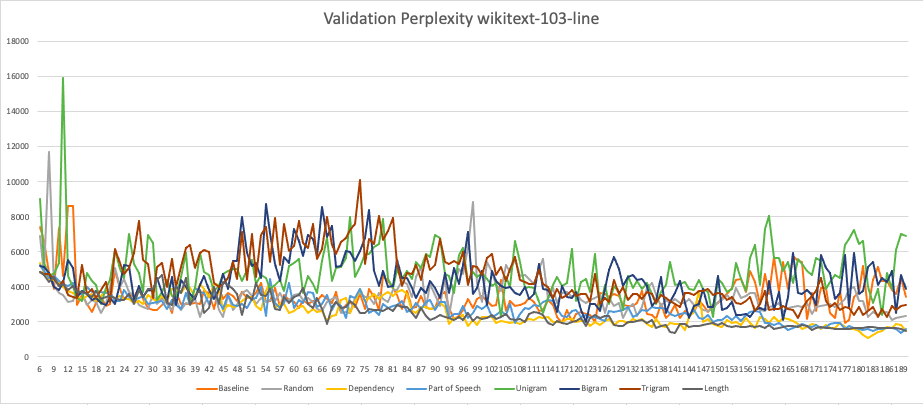
\includegraphics[width=10cm, height=10cm]{Thesis/images/wiki103-line-valid.png}
\caption{GLUE results for BS vs baseline.}
\end{figure}
\begin{table}[]
\centering
\resizebox{\textwidth}{!}{
\begin{tabular}{|l|l|l|l|l|l|l|l|l|}
\hline
Batches & Baseline & Random & Dependency & Part of Speech & Unigram & Bigram & Trigram & Length \\ \hline
0 & 133566.89 & 145170.9 & 157186.9 & 181081.6 & 145557 & 163357.2 & 154942.1 & 171047.1 \\  \hline
100 & 12285.347 & 11508.72 & 11214.37 & 16152.97 & 13442.27 & 11411.47 & 12175.73 & 14221.94 \\ \hline
200 & 6447.5767 & 6480.044 & 8555.388 & 7975.472 & 8173.018 & 7094.574 & 7406.791 & 7072.591 \\ \hline
300 & 5332.4336 & 5936.535 & 8272.807 & 6656.56 & 6980.953 & 5789.997 & 5697.248 & 6202.389 \\ \hline
400 & 5207.15 & 5223.892 & 5461.248 & 5642.629 & 5894.573 & 5175.929 & 5550.213 & 5249.547 \\ \hline
500 & 7429.528 & 6913.467 & 5345.27 & 5224.565 & 9022.917 & 5192.218 & 4844.931 & 4852.713 \\ \hline
600 & 6627.4604 & 4759.053 & 4770.627 & 4885.608 & 5370.834 & 5118.223 & 4742.507 & 4654.528 \\ \hline
700 & 4769.9443 & 11728.62 & 4452.612 & 4528.794 & 4650.765 & 4768.857 & 4716.095 & 4302.28 \\ \hline
800 & 3898.0117 & 4078.067 & 4383.075 & 4649.28 & 4734.933 & 3986.259 & 4436.026 & 4589.333 \\ \hline
900 & 7385.8477 & 3638.641 & 4217.924 & 4347.232 & 5342.706 & 3807.823 & 4032.682 & 4067.242 \\ \hline
1000 & 4610.644 & 3538.989 & 3972.509 & 4161.002 & 15954.95 & 4200.018 & 4312.525 & 4149.574 \\ \hline
1100 & 8622.547 & 3115.556 & 3737.612 & 4033.674 & 4617.307 & 5521.467 & 3553.627 & 3821.32 \\ \hline
1200 & 8631.456 & 3200.954 & 3666.757 & 4237.244 & 3974.965 & 5088.36 & 3428.275 & 4078.638 \\ \hline
1300 & 2980.604 & 3875.604 & 3463.381 & 3588.603 & 3340.407 & 3399.381 & 3372.226 & 3683.903 \\ \hline
1400 & 3539.7998 & 3630.569 & 3331.502 & 3611.937 & 3219.224 & 3757.146 & 5257.478 & 3687.256 \\ \hline
1500 & 3035.7773 & 2963.425 & 3455.519 & 3978.28 & 4819.782 & 3602.563 & 3591.551 & 3593.675 \\ \hline
1600 & 2589.6614 & 3252.407 & 3621.878 & 3732.493 & 4355.743 & 3276.338 & 3857.337 & 3438.57 \\ \hline
1700 & 3098.1157 & 3141.189 & 3216.005 & 3768.428 & 4081.203 & 3389.714 & 3384.101 & 3790.884 \\ \hline
1800 & 3428.1082 & 2522.237 & 3475.266 & 3735.106 & 3026.908 & 3103.072 & 3821.906 & 3335.825 \\ \hline
1900 & 2923.9253 & 3033.856 & 3818.332 & 3650.337 & 3948.062 & 2993.07 & 4274.857 & 3396.03 \\ \hline
2000 & 3024.5503 & 4015.455 & 3462.04 & 3686.353 & 4419.2 & 3353.64 & 3111.692 & 3499.381 \\ \hline
2100 & 4984.682 & 5106.585 & 3339.451 & 3206.319 & 6102.428 & 3008.452 & 6180.235 & 3381.545 \\ \hline
2200 & 3904.0237 & 4004.407 & 3499.03 & 3180.93 & 5009.597 & 4163.797 & 5390.852 & 3248.532 \\ \hline
2300 & 3326.3901 & 4438.087 & 3309.986 & 3827.221 & 4498.915 & 5244.173 & 4708.613 & 3237.241 \\ \hline
2400 & 3617.3625 & 3705.34 & 3321.961 & 3443.669 & 7043.6 & 5192.322 & 5087.759 & 3612.678 \\ \hline
2500 & 3426.1863 & 3493.156 & 3101.16 & 3278.573 & 5294.611 & 3262.285 & 5959.082 & 3029.704 \\ \hline
2600 & 3929.536 & 2989.818 & 3169.209 & 3348.961 & 4787.855 & 4064.311 & 7771.3 & 3839.325 \\ \hline
2700 & 3318.4084 & 2877.347 & 3041.625 & 3465.139 & 3686.567 & 3402.472 & 5554.846 & 3434.443 \\ \hline
2800 & 2798.2139 & 2729.84 & 3553.2 & 3015.829 & 6963.724 & 3806.571 & 5296.702 & 3893.353 \\ \hline
2900 & 2653.2427 & 3578.958 & 3330.19 & 3079.564 & 6497.482 & 3760.58 & 3342.895 & 3861.117 \\ \hline
3000 & 2671.6992 & 3000.713 & 3196.162 & 3112.699 & 3264.097 & 4493.842 & 5113.974 & 4389.064 \\ \hline
3100 & 2956.447 & 3357.973 & 3479.73 & 3169.381 & 3712.669 & 3669.551 & 5344.856 & 4664.851 \\ \hline
3200 & 3287.3135 & 3001.875 & 3196.72 & 2764.877 & 4382.15 & 3182.293 & 3989.385 & 3054.209 \\ \hline
3300 & 2486.855 & 2674.501 & 3894.077 & 3264.268 & 3460.631 & 4561.381 & 5568.212 & 2944.834 \\ \hline
3400 & 3681.2234 & 3264.878 & 3909.351 & 2989.094 & 3445.657 & 2945.227 & 3972.854 & 4048.585 \\ \hline
3500 & 3042.2605 & 2669.779 & 3652.555 & 2723.573 & 4546.983 & 4400.884 & 5114.647 & 3656.315 \\ \hline
3600 & 3042.0315 & 3091.007 & 4027.494 & 3650.473 & 5930.231 & 3982.463 & 6214.663 & 4501.413 \\ \hline
3700 & 3043.7842 & 3014.716 & 3912.738 & 3008.312 & 3147.093 & 3602.845 & 6376.496 & 2952.597 \\ \hline
3800 & 3102.6042 & 3313.633 & 3447.961 & 3930.166 & 3914.254 & 3298.151 & 5062.238 & 3494.175 \\ \hline
3900 & 3013.213 & 2299.637 & 4141.134 & 3733.276 & 5935.788 & 4126.57 & 5946.967 & 3836.997 \\ \hline
4000 & 3759.0522 & 2979.182 & 3887.857 & 3650.793 & 4862.929 & 4629.568 & 6099.234 & 2529.98 \\ \hline
4100 & 3668.0715 & 3541.252 & 3407.547 & 3026.772 & 4674.399 & 3848.662 & 5993.873 & 2789.232 \\ \hline
4200 & 2730.591 & 3756.239 & 4172.849 & 3658.614 & 3783.238 & 3288.383 & 4222.746 & 3993.321 \\ \hline
4300 & 3949.8096 & 2681.376 & 4080.428 & 3128.34 & 4029.699 & 3868.773 & 3971.199 & 3006.097 \\ \hline
4400 & 3323.0835 & 2296.129 & 2628.662 & 2761.743 & 4746.249 & 4753.029 & 4173.327 & 4290.566 \\ \hline
4500 & 3658.6946 & 3549.945 & 2943.47 & 3554.22 & 4932.861 & 3854.719 & 4499.232 & 4120.625 \\ \hline
4600 & 3498.2964 & 2664.737 & 2869.677 & 2947.416 & 5012.292 & 5464.019 & 5441.119 & 3875.83 \\ \hline
4700 & 3218.3953 & 2993.687 & 2914.067 & 2931.284 & 5009.84 & 5457.208 & 4473.262 & 3604.246 \\ \hline
4800 & 3705.17 & 3623.094 & 3179.02 & 3024.836 & 4351.454 & 7997.697 & 7150.244 & 2385.476 \\ \hline
4900 & 3371.4956 & 3825.662 & 3449.096 & 2820.489 & 4956.879 & 5906.345 & 4408.281 & 3551.005 \\ \hline
5000 & 3406.368 & 3478.585 & 3437.806 & 3316.647 & 5550.663 & 5213.405 & 7000.541 & 3251.957 \\ \hline
5100 & 3658.293 & 3001.878 & 2934.582 & 3339.919 & 4153.177 & 5386.484 & 4569.976 & 4214.997 \\ \hline
5200 & 4194.59 & 3349.578 & 2663.698 & 4014.084 & 4672.335 & 4513.1 & 6939.784 & 3541.404 \\ \hline
5300 & 3139.5151 & 3182.787 & 3781.348 & 2353.679 & 4483.329 & 8713.253 & 7396.936 & 3471.748 \\ \hline
5400 & 3214.4783 & 3224.414 & 4276.697 & 4426.463 & 3902.706 & 7097.28 & 5437.933 & 3852.584 \\ \hline
5500 & 3932.4114 & 3201.333 & 2812.856 & 3057.271 & 4108.582 & 5330.817 & 7914.916 & 2754.497 \\ \hline
5600 & 2864.2917 & 3627.737 & 3003.349 & 2815.709 & 4386.842 & 4327.014 & 5232.348 & 2702.415 \\ \hline
5700 & 3538.355 & 3176.168 & 3046.171 & 3060.973 & 3772.631 & 5686.305 & 7596.855 & 3421.795 \\ \hline
5800 & 3252.9683 & 3272.469 & 2486.868 & 4196.891 & 5201.184 & 5386.043 & 6068.738 & 3089.486 \\ \hline
5900 & 3131.4595 & 3539.543 & 2635.31 & 2772.455 & 5381.719 & 7309.636 & 6318.746 & 3442.756 \\ \hline
6000 & 2794.038 & 3587.836 & 2825.41 & 3244.816 & 5596.753 & 6640.867 & 7775.148 & 3509.842 \\ \hline
6100 & 3251.644 & 3263.527 & 2918.197 & 3100.223 & 3635.773 & 5764.608 & 6505.952 & 3940.546 \\ \hline
6200 & 3002.94 & 3363.021 & 2487.748 & 3734.48 & 4609.224 & 6966.229 & 6210.936 & 3022.155 \\ \hline
6300 & 3218.558 & 3161.412 & 2762.742 & 3631.77 & 4138.99 & 6753.394 & 7590.026 & 2781.639 \\ \hline
6400 & 3168.3445 & 2745.09 & 2539.634 & 2845.859 & 3643.194 & 5790.03 & 5593.007 & 3362.367 \\ \hline
6500 & 3563.9138 & 2631.605 & 2615.582 & 3017.273 & 5498.478 & 8534.298 & 6150.414 & 2755.562 \\ \hline
6600 & 3336.5125 & 3152.491 & 2045.112 & 3510.307 & 6806.122 & 6820.456 & 8015.877 & 1892.766 \\ \hline
6700 & 3095.4402 & 3280.077 & 2363.671 & 2707.773 & 4330.916 & 7460.527 & 6372.921 & 2842.231 \\ \hline
6800 & 3707.2769 & 3402.757 & 2401.957 & 3146.946 & 5093.779 & 5133.348 & 5852.205 & 3127.991 \\ \hline
6900 & 2563.3862 & 2491.408 & 3224.506 & 2928.696 & 5140.863 & 5176.373 & 6588.458 & 2814.376 \\ \hline
7000 & 2950.2212 & 2558.31 & 3351.246 & 2230.343 & 5639.729 & 6032.242 & 6812.246 & 2852.699 \\ \hline
7100 & 3118.5103 & 2508.693 & 2510.393 & 3488.994 & 7993.922 & 5985.55 & 7232.887 & 3199.032 \\ \hline
7200 & 2862.5986 & 3386.939 & 3137.043 & 3367.331 & 4575.148 & 5486.356 & 7562.751 & 2948.376 \\ \hline
7300 & 3581.2903 & 3661.634 & 3901.34 & 3907.249 & 5122.223 & 6055.366 & 10125.68 & 2535.578 \\ \hline
7400 & 2722.6355 & 3448.971 & 3190.647 & 3167.26 & 5884.57 & 6804.227 & 5294.717 & 2535.351 \\ \hline
7500 & 3889.6006 & 3437.576 & 3360.645 & 2520.448 & 5903.479 & 8383.122 & 6737.35 & 2751.326 \\ \hline
7600 & 3435.7764 & 3023.607 & 3594.426 & 2703.097 & 6273.879 & 4891.422 & 6465.556 & 2662.755 \\ \hline
7700 & 2684.486 & 3649.864 & 3326.815 & 2410.613 & 6438.52 & 4077.892 & 8025.103 & 2668.974 \\ \hline
7800 & 4623.788 & 3301.87 & 3548.683 & 3013.871 & 7893.651 & 4928.719 & 6681.804 & 2631.33 \\ \hline
7900 & 4340.479 & 3161.765 & 3719.331 & 2770.811 & 4452.123 & 3993.706 & 7188.245 & 2779.878 \\ \hline
8000 & 3961.5264 & 3807.014 & 3452.459 & 2907.043 & 3954.853 & 4021.901 & 7929.308 & 2643.695 \\ \hline
8100 & 3549.708 & 3812.812 & 3715.364 & 2949.986 & 4943.123 & 5520.156 & 5313.925 & 2967.196 \\ \hline
8200 & 2721.3855 & 4309.146 & 3804.868 & 3194.562 & 4426.138 & 4493.306 & 4023.474 & 2833.751 \\ \hline
8300 & 3770.7717 & 4154.175 & 3602.226 & 2562.071 & 4908.361 & 4478.966 & 4814.494 & 2852.929 \\ \hline
8400 & 2819.1184 & 3395.214 & 2647.107 & 2739.021 & 4440.539 & 3912.589 & 4741.123 & 2516.4 \\ \hline
8500 & 2855.0764 & 4537.215 & 2495.408 & 3064.236 & 5412.395 & 3348.591 & 5236.132 & 2208.325 \\ \hline
8600 & 3505.9644 & 5123.063 & 2870.41 & 2727.767 & 5053.71 & 3948.653 & 4403.252 & 2785.527 \\ \hline
8700 & 2836.03 & 2766.154 & 2849.205 & 3117.907 & 5864.273 & 3649.038 & 5827.049 & 2355.334 \\ \hline
8800 & 2745.462 & 4155.193 & 2720.012 & 3277.113 & 5727.051 & 4311.576 & 4987.207 & 2098.654 \\ \hline
8900 & 2791.9512 & 3517.63 & 2800.61 & 2664.944 & 6971.113 & 3963.825 & 5239.959 & 2229.124 \\ \hline
9000 & 3544.8262 & 2923.488 & 3053.754 & 3133.222 & 6793.178 & 3378.838 & 6722.614 & 2413.132 \\ \hline
9100 & 3718.3665 & 4568.477 & 2841.7 & 3127.884 & 4710.665 & 4798.744 & 5396.799 & 2281.898 \\ \hline
9200 & 2808.6433 & 2312.481 & 1903.869 & 2207.872 & 4649.204 & 3642.391 & 5320.887 & 2199.175 \\ \hline
9300 & 2165.4578 & 3975.026 & 2209.777 & 2472.435 & 3676.473 & 5090.67 & 5474.493 & 2135.631 \\ \hline
9400 & 2339.3792 & 5000.876 & 2221.992 & 2454.856 & 5797.444 & 4136.993 & 5279.44 & 2281.424 \\ \hline
9500 & 2696.5264 & 4750.741 & 2413.11 & 2918.894 & 6209.71 & 5272.023 & 6008.77 & 2130.816 \\ \hline
9600 & 3324.4998 & 6199.148 & 1773.672 & 2194.82 & 4300.943 & 7148.329 & 4094.777 & 2508.34 \\ \hline
9700 & 2773.0059 & 8854.468 & 2118.811 & 2509.108 & 4839.8 & 3611.947 & 5180.166 & 2075.662 \\ \hline
9800 & 3280.1736 & 4203.143 & 1835.579 & 2932.314 & 4556.438 & 3910.895 & 5137.227 & 2268.739 \\ \hline
9900 & 3473.049 & 3118.263 & 2283.341 & 2728.226 & 4778.486 & 4880.072 & 4650.047 & 2173.566 \\ \hline
10000 & 3186.8086 & 5426.308 & 2254.678 & 2943.919 & 4426.129 & 2952.908 & 5637.761 & 2230.848 \\ \hline
10100 & 2909.2644 & 4874.029 & 2301.296 & 2268.375 & 4064.935 & 4881.747 & 5865.94 & 2422.808 \\ \hline
10200 & 2970.3079 & 4136.014 & 1920.374 & 2401.191 & 4241.271 & 4340.136 & 4660.822 & 2176.211 \\ \hline
10300 & 4404.0874 & 3743.304 & 2076.806 & 2608.362 & 2282.178 & 4047.018 & 5157.879 & 2288.977 \\ \hline
10400 & 2650.5618 & 5259.514 & 1997.169 & 2377.451 & 4587.451 & 3908.919 & 4345.876 & 2457.326 \\ \hline
10500 & 3188.861 & 4863.026 & 1921.195 & 3030.305 & 3993.9 & 4020.728 & 5001.028 & 2137.973 \\ \hline
10600 & 2928.7676 & 5619.987 & 2021.615 & 1937.735 & 6627.106 & 3641.662 & 5715.097 & 2114.58 \\ \hline
10700 & 2990.6763 & 4632.581 & 1891.141 & 2465.603 & 5435.766 & 3554.868 & 4419.398 & 2176.237 \\ \hline
10800 & 3106.0146 & 4674.662 & 2052.121 & 2789.199 & 3919.651 & 4020.114 & 4256.856 & 1980.449 \\ \hline
10900 & 3359.8572 & 4426.294 & 2156.759 & 2719.192 & 4010.09 & 3295.575 & 4190.228 & 2470.908 \\ \hline
11000 & 3135.9302 & 4158.012 & 2085.822 & 2977.462 & 3938.63 & 3592.483 & 4167.802 & 2585.372 \\ \hline
11100 & 2600.6765 & 4998.616 & 2287.749 & 2902.101 & 3135.488 & 5292.259 & 4984.297 & 2497.218 \\ \hline
11200 & 2697.7224 & 5610.622 & 2237.043 & 3115.647 & 2486.967 & 3883.755 & 4174.605 & 2403.552 \\ \hline
11300 & 3249.2195 & 3319.064 & 2291.24 & 3233.927 & 3354.398 & 3823.685 & 3968.204 & 1961.928 \\ \hline
11400 & 2947.6704 & 3926.981 & 1995.444 & 3182.323 & 4094.028 & 3279.589 & 3376.812 & 1822.583 \\ \hline
11500 & 2266.9912 & 3061.715 & 1997.625 & 2737.797 & 4591.544 & 2559.695 & 3850.975 & 2051.783 \\ \hline
11600 & 1910.9951 & 3633.076 & 2017.666 & 2339.021 & 4046.791 & 4028.116 & 3389.805 & 1911.797 \\ \hline
11700 & 2703.9133 & 3730.606 & 2161.455 & 2292.595 & 4232.192 & 3396.06 & 3526.608 & 1887.096 \\ \hline
11800 & 1997.3059 & 3413.994 & 2171.736 & 2602.599 & 6137.459 & 3386.59 & 3847.157 & 2001.94 \\ \hline
11900 & 2472.8403 & 3623.55 & 2011.956 & 2686.452 & 3209.035 & 3684.933 & 3470.721 & 2055.052 \\  \hline
12000 & 2580.0857 & 3236.756 & 2047.223 & 2287.82 & 4252.911 & 2692.896 & 3619.992 & 2211.584 \\ \hline
12100 & 2462.5713 & 3107.209 & 2061.792 & 2409.757 & 4442.029 & 2022.006 & 3572.707 & 1738.626 \\ \hline
12200 & 2386.6958 & 3270.702 & 1742.09 & 2218.87 & 3714.259 & 3032.846 & 3149.919 & 2231.156 \\ \hline
12300 & 2010.5862 & 3375.562 & 1971.577 & 2276.157 & 5888.235 & 3010.039 & 4748.44 & 2376.187 \\ \hline
12400 & 3649.7207 & 3523.468 & 1807.192 & 2140.037 & 2789.801 & 2627.215 & 3046.564 & 2197.488 \\ \hline
12500 & 3616.9211 & 2527.415 & 2066.436 & 2079.851 & 4106.784 & 3907.022 & 3353.525 & 2315.153 \\ \hline
12600 & 3447.208 & 3352.406 & 2161.191 & 2616.749 & 2996.938 & 4944.613 & 3134.28 & 2356.557 \\ \hline
12700 & 3567.5286 & 2887.539 & 1850.102 & 2555.376 & 4026.019 & 5691.963 & 4392.883 & 1837.156 \\ \hline
12800 & 3496.0151 & 3070.08 & 2051.071 & 2613.339 & 3699.5 & 4996.399 & 3595.804 & 1779.349 \\ \hline
12900 & 2957.0505 & 2200.042 & 2029.144 & 2694.993 & 2655.597 & 4044.406 & 3979.509 & 1772.636 \\ \hline
13000 & 2889.5964 & 2821.793 & 1962.677 & 2848.288 & 4612.958 & 4555.686 & 3244.529 & 1971.573 \\ \hline
13100 & 2884.492 & 3042.716 & 2148.672 & 2278.382 & 3911.167 & 4696.947 & 3596.171 & 1991.141 \\ \hline
13200 & 3089.082 & 2329.917 & 2051.666 & 2415.661 & 4331.807 & 4364.996 & 3576.048 & 2060.151 \\ \hline
13300 & 3780.2158 & 2874.229 & 2148.193 & 2687.167 & 3905.77 & 4439.62 & 3330.12 & 2088.202 \\ \hline
13400 & 2475.67 & 3946.725 & 1880.399 & 2624.047 & 4216.894 & 4043.237 & 3692.884 & 1956.24 \\ \hline
13500 & 2391.5706 & 4227.497 & 1702.377 & 2825.495 & 3614.787 & 2928.353 & 3596.696 & 2102.339 \\ \hline
13600 & 2178.5073 & 3532.708 & 2186.421 & 2787.64 & 2999.277 & 3202.496 & 3107.828 & 1650.679 \\ \hline
13700 & 3008.851 & 2929.372 & 1758.434 & 2765.942 & 3707.263 & 4550.124 & 3509.052 & 1763.421 \\ \hline
13800 & 2215.242 & 3245.225 & 1685.312 & 2763.713 & 4098.856 & 2509.298 & 3393.489 & 1802.992 \\ \hline
13900 & 2460.976 & 3058.251 & 1958.757 & 2428.149 & 5447.126 & 3144.837 & 3197.692 & 1417.536 \\ \hline
14000 & 2944.5322 & 3279.467 & 1856.194 & 2358.343 & 4116.395 & 3639.197 & 3004.733 & 1386.126 \\ \hline
14100 & 2243.2942 & 3078.41 & 1875.342 & 2476.079 & 4168.629 & 4346.108 & 2838.907 & 1855.109 \\ \hline
14200 & 2629.6426 & 3068.33 & 1520.55 & 2496.886 & 4298.392 & 3075.109 & 3678.563 & 1891.769 \\ \hline
14300 & 2368.2566 & 3311.473 & 2274.057 & 2409.711 & 3852.69 & 2250.046 & 3635.187 & 1708.987 \\ \hline
14400 & 2550.2156 & 2957.337 & 2546.271 & 2676.356 & 3802.065 & 2900.622 & 3531.421 & 1751.901 \\ \hline
14500 & 3179.2258 & 2918.599 & 3736.432 & 2196.153 & 4384.977 & 3041.994 & 3737.262 & 1747.746 \\ \hline
14600 & 2960.2913 & 2671.386 & 1978.412 & 2186.668 & 3883.192 & 3858.036 & 3759.196 & 1799.298 \\ \hline
14700 & 2556.041 & 2622.209 & 2180.598 & 2400.547 & 3716.956 & 2847.02 & 3890.97 & 1868.855 \\ \hline
14800 & 2944.977 & 2724.473 & 1908.646 & 2003.582 & 2287.438 & 2827.39 & 3519.482 & 1935.015 \\ \hline
14900 & 3058.9365 & 3159.76 & 1791.704 & 2110.232 & 4458.922 & 4601.517 & 3644.684 & 1814.54 \\ \hline
15000 & 3373.5347 & 3268.794 & 1731.719 & 2115.681 & 4234.21 & 2655.245 & 3602.088 & 1910.209 \\ \hline
15100 & 3619.1846 & 3525.784 & 2091.911 & 2336.762 & 3716.094 & 2779.542 & 3231.95 & 1780.052 \\ \hline
15200 & 3959.872 & 3215.453 & 1916.56 & 2132.752 & 3879.117 & 3125.468 & 3430.319 & 1701.954 \\ \hline
15300 & 4391.342 & 3927.056 & 1975.358 & 2348.073 & 5354.714 & 2415.163 & 3068.784 & 1756.15 \\ \hline
15400 & 4431.6123 & 3377.846 & 1849.331 & 2047.901 & 4445.123 & 2385.826 & 3000.101 & 1726.074 \\ \hline
15500 & 3709.352 & 3503.648 & 2244.007 & 2412.537 & 3740.15 & 2438.061 & 3197.201 & 1730.452 \\ \hline
15600 & 4916.862 & 3641.964 & 1946.571 & 2569.364 & 5624.819 & 2265.686 & 3404.546 & 1756.93 \\ \hline
15700 & 4265.769 & 3650.713 & 1639.628 & 2648.778 & 6393.979 & 2677.095 & 2602.288 & 1705.534 \\ \hline
15800 & 3012.003 & 2658.754 & 2292.661 & 2545.123 & 4097.075 & 2777.115 & 3035.369 & 1756.578 \\ \hline
15900 & 4748.132 & 2635.553 & 2167.567 & 1949.89 & 7333.727 & 2663.09 & 3760.357 & 1672.691 \\ \hline
16000 & 3591.87 & 2848.635 & 1961.523 & 1914.378 & 8042.142 & 4309.771 & 2692.323 & 1816.02 \\ \hline
16100 & 5728.612 & 2913.521 & 2280.985 & 1848.195 & 5667.022 & 2690.273 & 2760.998 & 1578.525 \\ \hline
16200 & 3709.089 & 3093.82 & 2017.133 & 1913.861 & 5655.845 & 3693.841 & 2730.397 & 1663.372 \\ \hline
16300 & 5435.975 & 2588.199 & 2200.272 & 1741.35 & 4931.408 & 2095.966 & 2910.535 & 1691.521 \\ \hline
16400 & 3899.814 & 2816.65 & 2143.566 & 1520.613 & 5432.34 & 3398.078 & 2736.456 & 1738.191 \\ \hline
16500 & 5760.409 & 2858.464 & 2046.358 & 1679.481 & 4213.457 & 5952.215 & 2700.678 & 1779.349 \\ \hline
16600 & 5474.128 & 2884.826 & 1884.325 & 1786.089 & 5583.255 & 3653.356 & 2235.502 & 1701.01 \\ \hline
16700 & 5394.362 & 2830.033 & 1613.511 & 1855.339 & 5332.088 & 3604.594 & 2763.783 & 1802.436 \\ \hline
16800 & 2142.807 & 3056.592 & 1726.021 & 1743.585 & 4894.997 & 3832.360 & 3168.774 & 1777.959 \\ \hline
16900 & 3653.911 & 2477.513 & 1876.478 & 1717.887 & 4702.398 & 3547.463 & 3506.964 & 1538.599 \\ \hline
17000 & 2623.699 & 2864.975 & 1814.027 & 1837.478 & 5624.287 & 2961.518 & 3777.023 & 1642.067 \\ \hline
17100 & 3946.361 & 2881.194 & 1573.796 & 1626.424 & 5477.412 & 5801.621 & 4522.428 & 1686.476 \\ \hline
17200 & 3931.53 & 2960.243 & 1825.012 & 1729.626 & 3872.457 & 5079.338 & 3204.623 & 1665.452 \\ \hline
17300 & 2483.086 & 3014.486 & 1674.596 & 1863.654 & 4254.981 & 4786.290 & 2864.236 & 1625.513 \\ \hline
17400 & 2201.756 & 2845.112 & 1661.79 & 1918.791 & 4660.876 & 3303.216 & 3083.025 & 1623.081 \\ \hline
17500 & 3762.044 & 3017.391 & 1963.165 & 1948.196 & 4514.555 & 3630.837 & 2700.909 & 1610.702 \\ \hline
17600 & 1916.478 & 3334.092 & 1713.173 & 1566.398 & 6403.468 & 5796.097 & 2827.983 & 1589.058 \\ \hline
17700 & 2133.296 & 3893.108 & 1615.585 & 1793.384 & 6750.477 & 2867.517 & 2806.61 & 1594.783 \\ \hline
17800 & 3443.813 & 4011.528 & 1590.357 & 1629.844 & 7231.735 & 5932.110 & 2400.474 & 1675.2 \\ \hline
17900 & 3704.21 & 3190.787 & 1469.256 & 1593.947 & 6466.648 & 3567.406 & 2875.86 & 1626.964 \\ \hline
18000 & 5203.719 & 3181.392 & 1228.67 & 1533.493 & 6644.731 & 3736.544 & 2382.266 & 1669.715 \\ \hline
18100 & 2668.049 & 2297.651 & 1099.461 & 1610.487 & 3970.642 & 5157.464 & 2630.59 & 1716.483 \\ \hline
18200 & 4370.502 & 2572.062 & 1273.885 & 1482.608 & 3078.424 & 5397.142 & 2872.213 & 1694.746 \\ \hline
18300 & 5140.358 & 2410.223 & 1444.652 & 1588.948 & 3883.507 & 4110.709 & 2288.334 & 1652.913 \\ \hline
18400 & 4342.102 & 2519.764 & 1502.864 & 1594.955 & 2383.756 & 4526.784 & 2733.952 & 1639.476 \\ \hline
18500 & 4314.982 & 2582.652 & 1734.776 & 1653.818 & 4777.05 & 4260.981 & 2298.712 & 1679.498 \\ \hline
18600 & 3823.823 & 2107.931 & 1651.656 & 1625.005 & 3894.389 & 4925.690 & 2919.162 & 1657.156 \\ \hline
18700 & 3579.227 & 2221.069 & 1889.513 & 1596.393 & 6128.305 & 2497.559 & 2705.167 & 1640.252 \\ \hline
18800 & 4485.336 & 2294.088 & 1851.501 & 1382.937 & 7034.37 & 4672.204 & 2903.462 & 1601.016 \\ \hline
18900 & 3450.497 & 2346.806 & 1466.698 & 1575.33 & 6894.88 & 3873.480 & 2945.7 & 1504.928 \\ \hline
\end{tabular}
}
\caption{wikitext-103-sentence}
\label{tab:wikitext-103-sentence}
\end{table}
\begin{figure}[h]
\centering
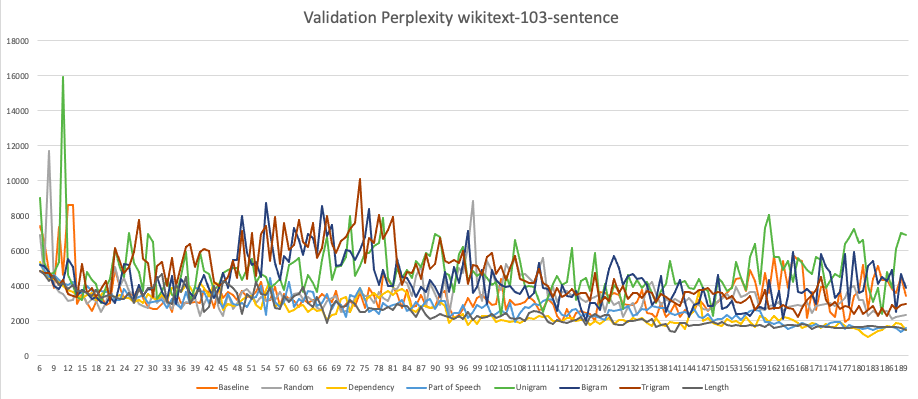
\includegraphics[width=10cm, height=10cm]{Thesis/images/wiki103-sentence-valid.png}
\caption{GLUE results for BS vs baseline.}
\end{figure}
\section{Discussion}
Looking at the results to our experiments we find it useful to formulate CL as moving from sampling without replacement to sampling with replacement with an ever growing population. As a result a fundamental difference is our implementations of CL do not guarantee that the model will actually see the entire dataset 10 times and as a result the distribution of the see train dataset is not representative validation dataset. While this is partially expected as the training task is auto regressive which is optimal for generation while the evaluation transfer task is understanding based, which is closer to auto encoding. We believe this is why the CL implementations are never able to generalize their performance in the train portion of the corpus to the validation portion. This finding is interesting because it challenges the notion that to learn a representation that transfers well to downstream tasks a model must fit the target dataset well. Actually we find that even the models with really high validation perplexities are still able to learn good representations for our transfer task. \\
Another observation our data leads us to is how the tweaking of the training distribution can allow the models to do better in transfer tasks because it is unable to overfit to the small data. Since our implementation generates some notion of continually random batches the train distribution is continually changing and thus it becomes harder for the model to overfit when compared to the static baseline sampling. It is our belief that CL is essentially acting as a method of representing a larger dataset than that which is used to train. We believe this is a potentially powerful observation which we would like to explore further down the line. \\
Additional observations we make from our data is there is no marked difference the effects of training with sentence based corpuses vs that of line based corpuses. This is matched with no immediately visible superior curricula heuristic makes us believe that language models learn more from the random distribution of a textual corpus than any structure experimenters try to introduce. Our experiments in many ways show how robust and efficient regular stochastic sampling is. The cost of shuffling happens once instead of every batch and no additional work needs to go to crafting the curricula.\\
Circling back on the questions we asked in our methodology section with regards to the CL methods we implemented. 
\begin{enumerate}
\item CL can help converge to a more optimal global minima when the training corpus is small. As corpus size scales the positive impact of CL disappears.
\item The downstream representation learned via CL outperforms non curricula methods when the corpus size is small but as the corpus size grows CL methods no longer generate the best representation.
\item CL methods do not help the model convergence speed in any noticeable way.
\end{enumerate}